\chapter{Popis simulačného modelu}
\indent\indent Simulátor MiXiM sa v čase písania tejto práce vyvíjal relatívne dynamicky. Avšak v~podobe, v ktorej sa nachádzal, ešte neumožňoval plnohodnotnú prípravu modelu a dynamika jeho vývoja bola skôr na príťaž ako na osoh. To bol hlavný motív, prečo zostať pri Mobility Framework rozšírení. Našou snahou teda bolo pripraviť taký modul, ktorý sa bude dať vo vhodnej chvíli ľahko transformovať do podoby vhodnej pre simulačný framework MiXiM.\\
\indent Toto sa podarilo tak, že fyzickú vrstvu sme rozdelili na 2 časti. Jedna je napísaná spôsobom, aby vedela spracovávať formáty správ definované IEEE 802.15.4b-2006 štandardom, aby sekvencie udalostí, ktoré v nej prebiehajú, boli zodpovedajúce štandardu. Táto vrstva ale nekomunikuje priamo s modulom \ttfamily ChannelControl\rmfamily, ale predá správy druhej časti fyzickej vrstvy, a tá už je implementovaná v podobe, ktorá silno závisí na konkrétnom použitom rozšírení modulu OMNeT++. Medzi týmito dvoma základnými časťami komunikácia prebieha vo forme oznamov cez modul \ttfamily Blackboard \rmfamily a aj cez predávanie správ pomocou komunikačných brán. Komunikácia pomocou definovaných brán medzi uvedenými úrovňami fyzickej vrstvy sa deje výhradne za účelom preposielania správ na médium, alebo príjmu správ z prijímača.\\
\indent Aby sa zabezpečilo bezproblémové nasadenie mobility architektúry a prenos IP paketov sieťou IEEE 802.15.4, implementovali sme robustný model fyzickej a linkovej vrstvy. V zásade sme dodržali členenia na vrstvy tak, ako ho prezentuje štandard. To znamená implementovali model fyzickej (PHY) a linkovej (MAC) vrstvy z dokumentu IEEE 802.15.4~\cite{ieee06} a sieťová vrstva (NET) a aplikačná (APP) je pripravená podľa dokumentu Zig\-Bee Specification~\cite{zigbee08}. Medzi týmito vrstvami sú preposielané správy, ktoré sa v~podstate delia do dvoch základných skupín:\\
\begin{itemize}
 \item správy, obsahujúce užitočné dáta aplikácii
 \item správy, ktoré majú riadiaci charakter
\end{itemize}
\indent\indent Charakter komunikácie medzi jednotlivými vrstvami a návrh rozdelenia PHY vrstvy je vyobrazený na obr.~\ref{fig:architecture_model}.\\
\begin{figure}[htbp]
\begin{center}
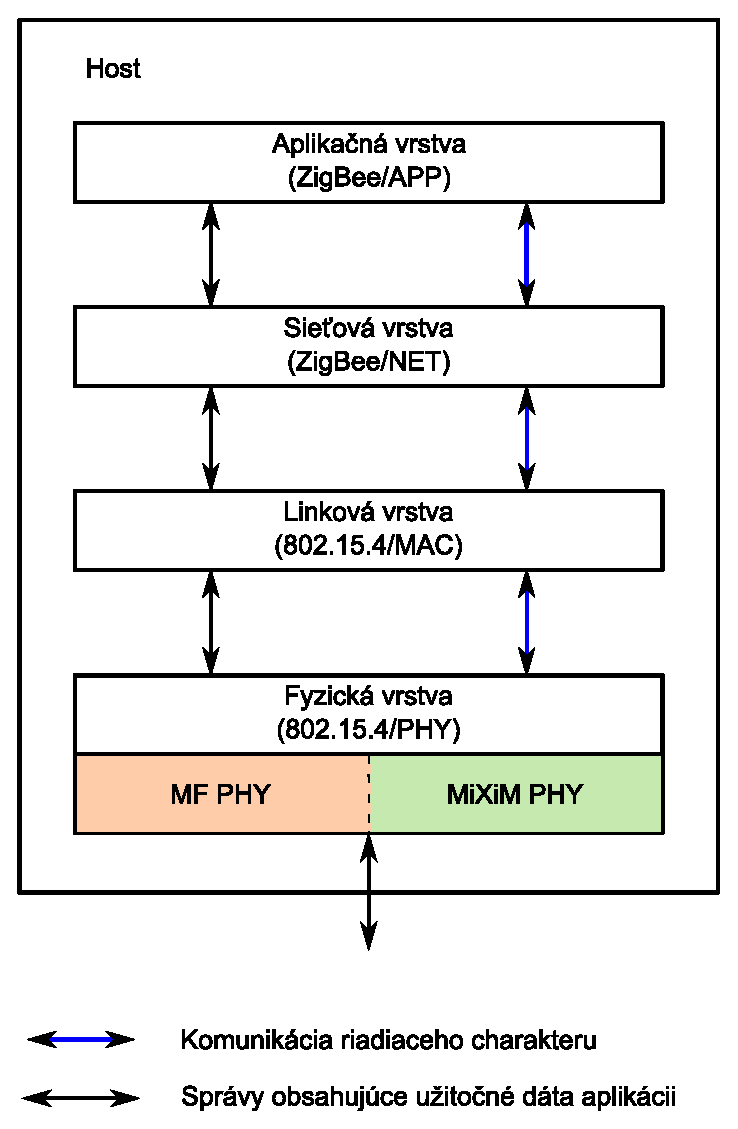
\includegraphics[width=120mm]{figures/architecture_model}
\caption{Základný pohľad na nami navrhovaný simulačný model}
\label{fig:architecture_model}
\end{center}
\end{figure}
\indent\indent Štruktúra jednotlivých vrstiev modelu sa ďalej člení na isté bloky, ktoré na každej z týchto vrstiev pracujú s presne definovanými správami. Jeden blok má na starosti spracovávanie riadiacich informácii, druhá časť vrstvy správy enkapsuluje pri postupe informácie v smere nadol v hierarchii vrstiev (dekapsuluje pri smere nahor). Oba tieto bloky samozrejme medzi sebou komunikujú. Ako tretí prvok v tejto štruktúre je databáza konfiguračných premenných, z ktorých časť má charakter konštánt a má teda dovolený len prístup na čítanie. K ostatným je povolený aj zápis, samozrejme len v~rámci medzí hodnôt, ktoré dovoľujú štandardy.\\
\indent Z ďalších vecí je zahrnutá podpora pre FFD a RFD zariadenia. Úloha uzlov je diverzifikovaná na úrovni aplikačnej vrstvy.\\

\section{Aplikačná vrstva - APP}
\indent\indent Čo sa týka aplikačnej vrstvy, mala by obsahovať vrstvu podpornú aplikačnej vrstvy (APSDE). Tú sme vynechali z dvoch dôvodov. Prvým a najdôležitejším, je ten, že nachádzame sa v oblasti, ktorej podoba silne závisí od výrobcov zariadení (OEM - Original Equipment Manufacturer) a konkrétnych účelov, pre ktoré bolo ZigBee zariadenie vyrobené. Druhým je, že pri získavaní dát o kvalite a rýchlosti algoritmov, ktoré najviac ovplyvňujú a charakterizujú siete ZigBee nemá aplikačná vrstva veľkú váhu. Aplikačná vrstva v nami danej podobe má úlohu spustiť procesy pre zmonitorovanie prostredia, pre zostavenie PAN siete. V ďalšom kroku povolí na nami definovaný interval (akceptuje sa aj nekonečne dlhý interval - hodnota premennej \textit{permitDuration} $0xFF$) FFD zariadeniam asociovať ďalšie prvky do siete.\\

\section{Sieťová vrstva - NET}
\indent\indent Sieťová vrstva je členená bloky (obr.~\ref{fig:topology_net}), každý z nich si plní svoje špecifické úlohy. Funkcie týchto blokov zodpovedajú ich popisu v ZigBee špecifikácii. Od sieťovej vrstvy sa požaduje poskytovanie funkcionality a zaistenie vhodných služieb pre správne fungovanie IEEE 802.15.4b-2006 linkovej vrstvy. K rozhraniu smerom k aplikačnej vrstve, ponúka koncept sieťovej vrstvy služby dvoch funkčných blokov. Tieto bloky sú označované ako datová (NLDE - Network Layer Data Entity) a riadiaca (NLME - Network Layer Management Entity).\\
\begin{figure}[htbp]
\begin{center}
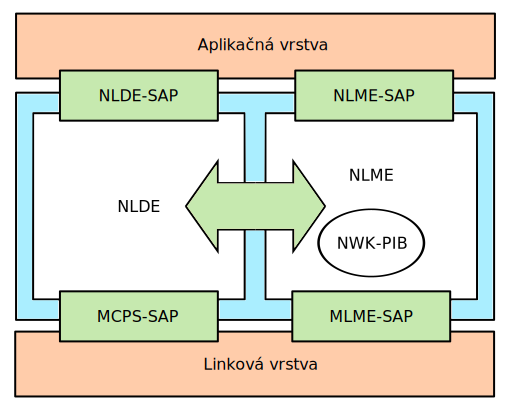
\includegraphics[width=120mm]{figures/topology_net}
\caption{Referenčný model sieťovej vrstvy}
\label{fig:topology_net}
\end{center}
\end{figure}
\subsection{Datová entita - NLDE}
\indent\indent Blok NLDE  (Network Layer Data Entity) poskytuje datové služby, ktoré dovolia aplikácii prenos im vlastných datových jednotiek (APDU - Application Protocol Data Unit) medzi viacerými zariadeniami na jednej PAN sieti. V princípe NLDE poskytuje služby:
\begin{itemize}
\item Vytváranie a spracovávanie datových jednotiek sieťovej vrstvy (NPDU - Network level PDU)
\item Smerovanie NPDU cieľovému zariadeniu v závislosti od topológie
\item Zaistenie autentizácie a utajenia prenosu, ak je vyžadované
\end{itemize}
\subsection{Riadiaca entita - NLME}
\indent\indent Riadiaca entita sieťovej vrstvy NLME (Network Layer Management Entity) podľa špecifikácie vykonáva tieto úlohy:
\begin{itemize}
\item Konfigurácia nových zariadení
\item Založenie novej siete
\item Pripájanie sa do existujúcich sietí (či už v rámci štartovacej sekvencie zariadenia, alebo po osirotení)
\item Prideľovanie 16-bitových adries podľa zabudovaného algoritmu
\item Udržovanie si zoznamu susediacich prvkov v dosahu rádia
\item Dáva k dispozícii viaceré smerovacie algoritmy v závislosti od charakteru vyžadovaného prenosu (unicast, multicast, broadcast)
\end{itemize}
\paragraph{Implementácia}
Implementácia sieťovej vrstvy počíta s rozdelením na 3 jednoduché moduly v jazyku NED. Tieto budú NLME, NLDE a NWK-PIB (Network layer Protocol Information Base). Moduly NLME a NLDE budú pripojené pomocou párov jednosmerných brán k~aplikačnej vrstve. Takisto sa počíta so zasielaním správ priamo medzi modulmi NLME a NLDE, preto aj v tomto mieste bude otvorená komunikačná cesta. Ako tretí bude jednoduchý modul NWK-PIB. Tento nebude pripojený k žiadnemu inému modulu komunikačnými bránami, ale bude obsahovať nadefinované verejne prístupné metódy (\texttt{public}) slúžiace na zapisovanie hodnôt atribútov a čítanie hodnôt atribútov a konštánt pre sieťovú vrstvu.\\
\indent Vrstva NLME tiež obsahuje datovú štruktúru reprezentujúcu mapu susediacich prvkov \texttt{std::map<unsigned long, NeighborTableEntry>}. Každý z týchto prvkov je identifikovaný 64-bitovým kľúčom - IEEE adresou. Záznam v tabuľke \texttt{NeighborTableEntry} obsahuje polia tak, ako sú pre tabuľku susedov definované v ZigBee špecifikácii.\\
\indent Ďalej si modul NLME uchováva aj informácie o PAN sietiach vo svojom okolí a v prípade FFD prvku tiež zaznamenáva počet asociovaných potomkov do siete a ich charakter (koncové zariadenie/smerovač) pre správne fungovanie distribuovaného mechanizmu prideľovania sieťových adries. Ak si zariadenie ukladá do \textit{neighborTable} záznam o smerovači, tak v tomto zázname je obsiahnutá aj informácia \textit{incomingBeaconTimestamp}, ktorá hovorí o relatívnej dobe prijatia beacon rámca od daného zariadenia. Hodnota je udaná v symboloch. Mimo to záznam v tabuľke, obsahuje ešte údaj v symboloch o~časovom odstupe beacon rámca vysielaného susediacim prvkov a prijímaného susediacim prvkom od jeho rodiča v topológii siete. Vďaka kombinácii týchto dvoch údajov si vie potom ďalší prvok účinne naplánovať vysielanie beacon rámcov tak, aby nespôsobovalo konflikty s inými beacon rámcami.\\
\indent Sieťová vrstva cez svoj modul NLME zapisuje do MAC-PIB (Medium Access Control layer Protocol Information Base) modulu linkovej vrstvy cez primitívu MLME-SET.request časť obsahu beacon rámcov označovanú ako \textit{macBeaconPayload}. Sú to informácie pre sieťové vrstvy susediacich prvkov, ktoré sú podávané cez implementovanú komunikačnú primitívu MLME-BEACON-NOTIFY.indication.\\
\indent K týmto trom základným blokom (NLDE, NLME, NWK-PIB) je pridaný blok \textit{Arp}. Idea tohoto riešenia je v separovaní smerovacieho algoritmu v extra module z dôvodu jeho prehľadnejšieho ladenia a ľahkosti v prípadnom experimentovaní s použitím iných smerovacích algoritmov.\\
\begin{figure}[htbp]
\begin{center}
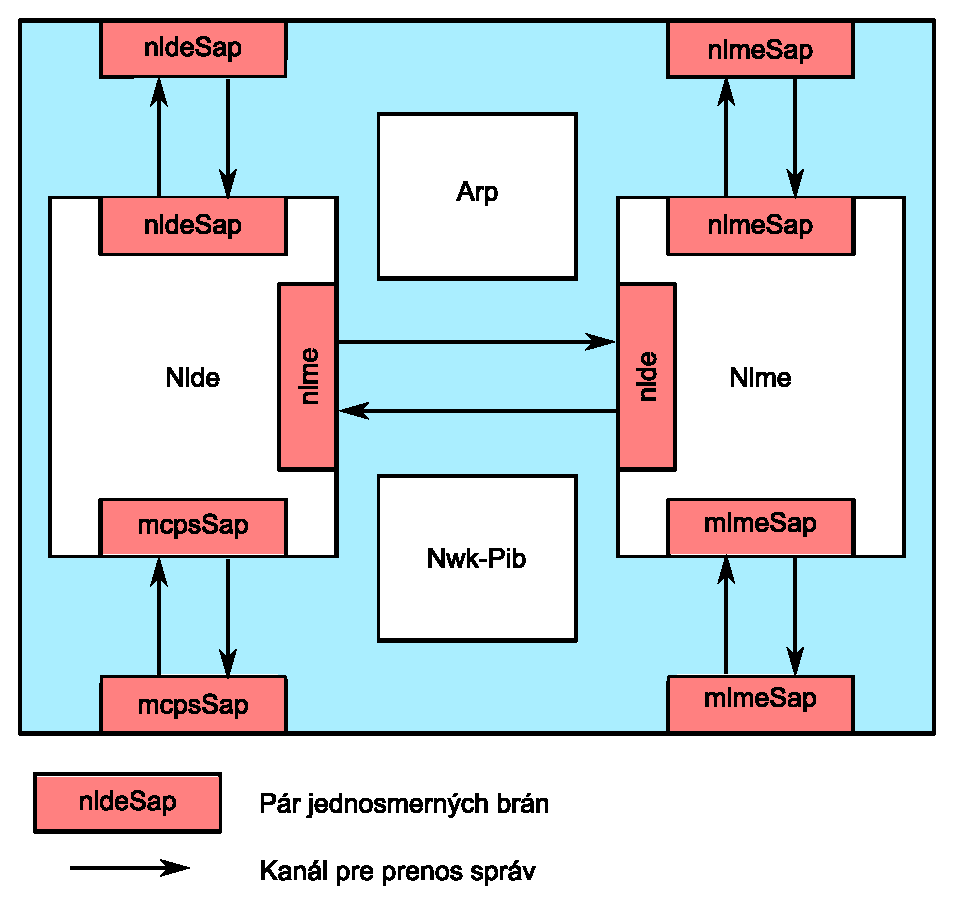
\includegraphics[width=120mm]{figures/architecture_net}
\caption{Podoba implementovaného modelu sieťovej vrstvy}
\label{fig:architecture_net}
\end{center}
\end{figure}

\section{Linková vrstva - MAC}
\indent\indent Úlohou linkovej vrstvy je riadiť prístup na prenosové médium a spracovávať informácie prijaté rádiom. V prípade linkovej vrstvy sú entity použité tiež dve - datová (MCPS - MAC Common Part Sublayer) a riadiaca (MLME - MAC Layer Management Entity). Okrem toho, že ponúkajú služby sieťovej vrstve cez príslušné body služby (SAP), existuje medzi nimi rozhranie, ktoré zabezpečuje riadiacej MLME entite využívať datové služby entity MCPS. Linková vrstva dokáže pracovať v 2 režimoch - beacon enabled a~non-beacon enabled móde. V prípade beacon-enabled módu prvok v roli smerovača v pravidelných intervaloch vysiela beacon rámec. Periodicita vysielania tohoto rámca je daná hodnotou premennej \textit{macBeaconOrder}. V prípade hodnoty $macBeaconOrder = 0x0F$ pracuje sieť v non-beacon enabled móde a beacon rámce sú zasielané len na vyžiadanie. V našom modeli sme sa vyhli implementácii tohoto módu, pretože podobné implementácie v simulátore OMNeT++ už existujú. Mimo to, úlohy linkovej vrstvy sú delené do dvoch skupín v závislosti od funkcionality, ktorá je od nich požadovaná:
\paragraph{FFD funkcionalita}
\begin{itemize}
\item Fungovanie v akejkoľvek topológii
\item Schopnosť fungovať v roli PAN koordinátor
\item Schopnosť komunikovať s akýmkoľvek IEEE 802.15.4 zariadením v PAN sieti
\item Implementovaná kompletná sada protokolu IEEE 802.15.4
\end{itemize}
\paragraph{RFD funkcionalita}
\begin{itemize}
\item Funkcia obmedzená na hviezdicovú topológiu, alebo rolu end-device v peer-to-peer móde
\item Nemožnosť vytvoriť sieť a stať sa PAN koordinátorom
\item Komunikácia len s FFD zariadením
\item Jednoduchá implementácia
\item Nízka spotreba energie
\end{itemize}
\begin{figure}[htbp]
\begin{center}
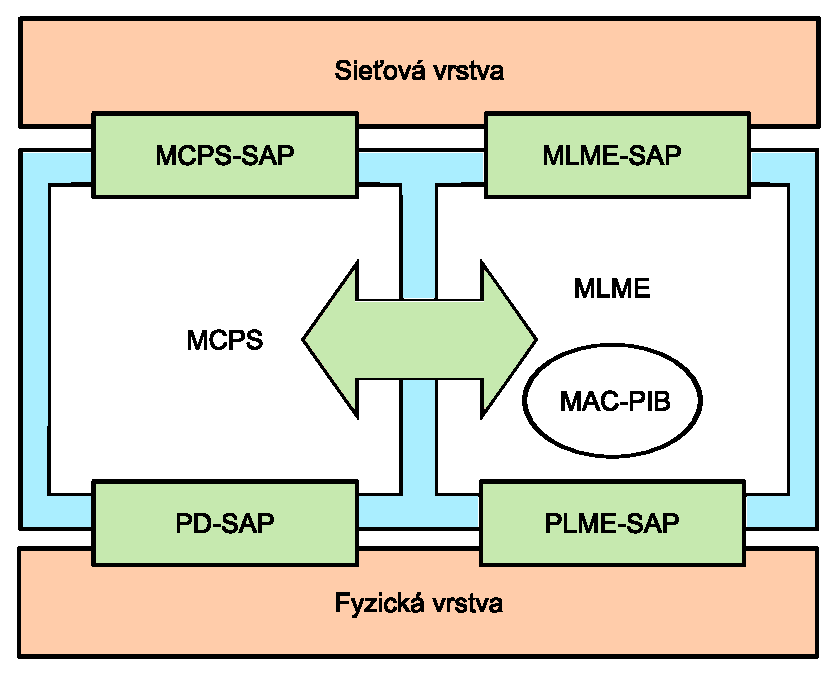
\includegraphics[width=120mm]{figures/topology_mac}
\caption{Referenčný model linkovej vrstvy}
\label{fig:topology_mac}
\end{center}
\end{figure}
\indent\indent Všetky zariadenia komunikujú na linkovej úrovni pomocou 64-bitových IEEE adries, alebo 16-bitových adries pridelených sieťovou vrstvou. Každá PAN sieť má pridelený svoj exkluzívny identifikátor. Tento identifikátor v kombinácii s cieľovou adresou definuje príjemcu komunikácie. Hodnota 16-bit sieťového identifikátora $0xFFFF$, alebo hodnota 16-bit PAN identifikátora $0xFFFF$ predstavuje broadcast adresu. Prijatý rámec, ktorý obsahuje takýto cieľový PAN identifikátor, alebo cieľovú sieťovú adresu nie je zahodený a je spracovaný linkovou vrstvou. Kontrola toho, či dané zariadenie je adresátom prijatého rámca, je vykonávaná vo vrstve MCPS.\\
\subsection{Datová entita - MCPS}
\indent\indent Modul MCPS slúži na prenos SPDU (SSCS Protocol Data Unit) medzi viacerými SSCS entitami.\\
\paragraph{Implementácia}
Datová entita MCPS využíva pre prenos rámcov fronty. Naša implementácia používa tieto fronty dve. Jednu pre prenos správ v perióde CAP pri beacon enabled móde alebo pre prenos riadiacich správ s vyššou prioritou v non-beacon enabled móde a druhú pre prenos správ v móde non-beacon enabled, ktoré majú nižšiu prioritu. Do týchto front sú rámce vkladané hneď po zapúzdrení (enkapsulácii). Teda vrstva MCPS sa stará aj o~enkapsuláciu. Niekedy nemá potrebné informácie k enkapsulácii rámca, ktorý je poslaný z~povedzme NLME vrstvy, vtedy NLME využije datovej štruktúry \texttt{nextEncapsulation} a~nastaví v nej príslušné hodnoty. To sa týka parametrov, ktoré nie sú obsiahnuté v správach generovaných NLME vrstvou, ale sú potrebné pre korektnú enkapsuláciu daného paketu (obr.~\ref{fig:frame_mac}). Simulačný model sa nezaoberá bezpečnosťou, preto je pole Auxiliary Security Header vždy dĺžky $0$.\\
\indent Modul MCPS posiela rámce potvrdení, ak sú vyžadované. Používa k tomu časovač \textit{ackTimer}. Modul MCPS ďalej dodržiava časové odstupy medzi datovými rámcami a~ACK rámcami. Sú to intervaly dané štandardom, ktoré dávajú zariadeniam čas na spracovani prijatých rámcov. Spôsob dodržovania týchto odstupov je vyobrazený na obr.~\ref{fig:interframe_spacing}.\\
\begin{figure}[htbp]
\begin{center}
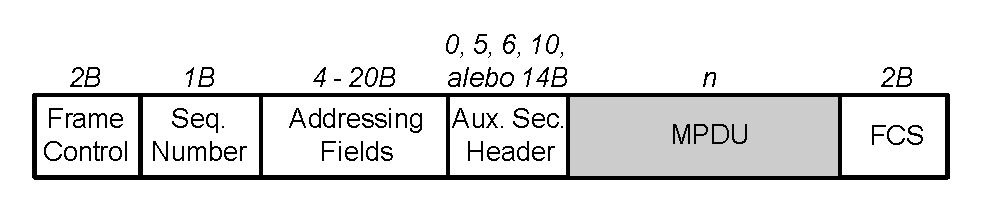
\includegraphics[width=140mm]{figures/frame_mac}
\caption{Spôsob enkapsulácie MPDU na linkovej vrstve}
\label{fig:frame_mac}
\end{center}
\end{figure}
\begin{figure}[htbp]
\begin{center}
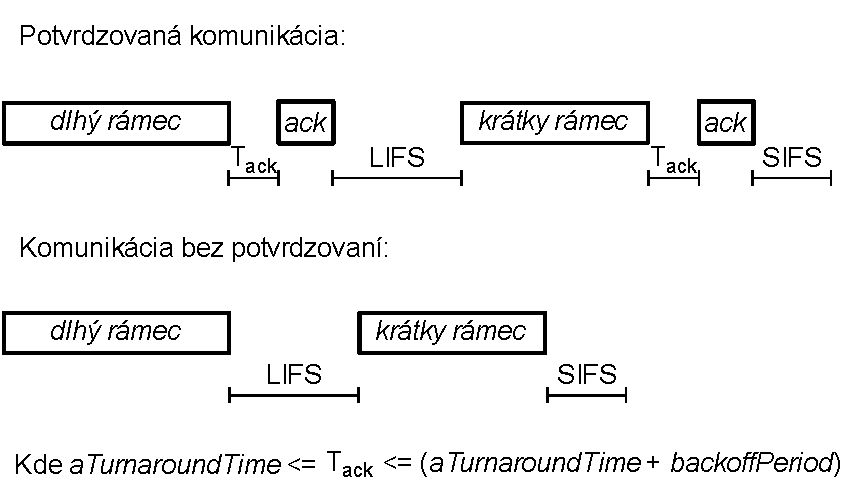
\includegraphics[width=120mm]{figures/interframe_spacing}
\caption{Minimálne časové odstupy medzi jednotlivými rámcami}
\label{fig:interframe_spacing}
\end{center}
\end{figure}
\subsection{Riadiaca entita - MLME}
\indent\indent MLME vrstva v časovom intervale označovanom ako CFP (viď obr.~\ref{fig:superframe}) realizuje prístup na médium cez tzv. CSMA-CA mechanizmus. CSMA mechanizmus znižuje pravdepodobnosť kolízie rámcov pri vysielaní viacerých rádii na spoločnom prenosovom médiu. Konkrétna aktivita CSMA mechanizmu sa nastavuje týmito parametrami:
\begin{itemize}
\item \textit{backoffExponent} (východzia hodnota: \textit{macMinBE})
\item \textit{numberOfBackoffs} (východzia hodnota: $0$)
\end{itemize}
\indent\indent CAP perióda je delená do 16 rovnako dlhých superframe slotov. Procedúra pre zistenie, či sa médium nachádza v stave \textit{idle} sa označuje ako Clear Channel Assessment (CCA) a vždy začína spolu so začiatkom nového superframe slotu. Prvý superframe slot je dedikovaný vysielaniu beacon rámca. Požiadavka na vysielanie rámca pomocou CSMA-CA mechanizmu začína po prvý krát vždy počas prvého superframe slotu. Keďže počas neho je vysielaný beacon rámec, CCA procedúra procedúra zistí, že kanál nie je voľný a začína tzv. backoff interval. Tento backoff interval hovorí o počte uplynutých superframe slotov pred ďalším pokusom o vyslanie rámca. Vypočíta sa ako náhodné číslo z intervalu $<0, 2^{backoffExponent})$. Po neúspešnom pokuse o vyslanie rámca sa zvýši hodnota \textit{backoffExponent} o jednotku a hodnota \textit{numberOfBackoffs} tiež o jednotku. Proces končí buď úspešným vyslaním rámca, prípadne dosiahnutím hraničných hodnôt $backoffExponent=macMaxBE$, alebo $numberOfBackoffs=macMaxCSMABackoffs+1$. Vtedy MLME vrstva vracia informáciu sieťovej vrstve so statusom \textit{channel failure}.\\
\indent Iba dva typy rámcov pristupujú v CAP intervale na médium bez aplikovania CSMA módu, a to sú rámce potvrdení (ACK frames) a beacon rámce.\\
\paragraph{Implementácia}
V prípade, že vyprší \textit{backoffTimer} v intervale CAP, MLME vrstva požiada PLME vrstvu primitívou PLME-CCA.request o vykonanie procedúry CCA aby mohlo začať vysielanie rámcov z vrstvy prioritnej fronty MCPS. Ak je prioritná fronta prázdna, pozrie sa na obsah druhej fronty. Možno by niekto mohol mať obavy, či takýto postup nespôsobí hladovanie (starving). Takto by sa dal označiť stav, kedy by sa prioritná fronta nikdy úplne nevyprázdnila a rámce v neprioritnej fronte by čakali teoreticky nekonečne dlho na odoslanie. V prípade architektúry siete 802.15.4 sa toho netreba obávať, pretože prioritná fronta sa využíva len zriedka, a to pre riadiace rámce MAC vrstvy (MAC Command frame) ako je napríklad žiadosť o vyslanie beacon rámca, žiadosť o asociáciu, o zistenie stavu asociácie, žiadosť o zaslanie dát smerom od smerovača a pod.\\
\indent Modul funguje ako stavový automat. Pre definovanie konkrétneho stavu v~ktorýkoľvek moment sú nám pomocné nasledovné premenné:
\begin{itemize}
\item \textit{lastUpperMsg} - premenná, ktorá uchováva kópiu posledne prijatej správy z vyššej vrstvy.
\item \textit{lastLowerMsg} - premenná, ktorá uchováva kópiu posledne prijatej správy z nižšej vrstvy, zatiaľ je používaná len v module (MLME).
\item \textit{layerStage} - v prípade, že vyššie uvedené štruktúry nedefinujú presne daný stav automatu, pomôže hodnota tejto premennej, po prijatí novej správy z vyššej vrstvy sa hodnota \textit{layerStage} nastavuje automaticky na $0$.
\end{itemize}
\begin{figure}[htbp]
\begin{center}
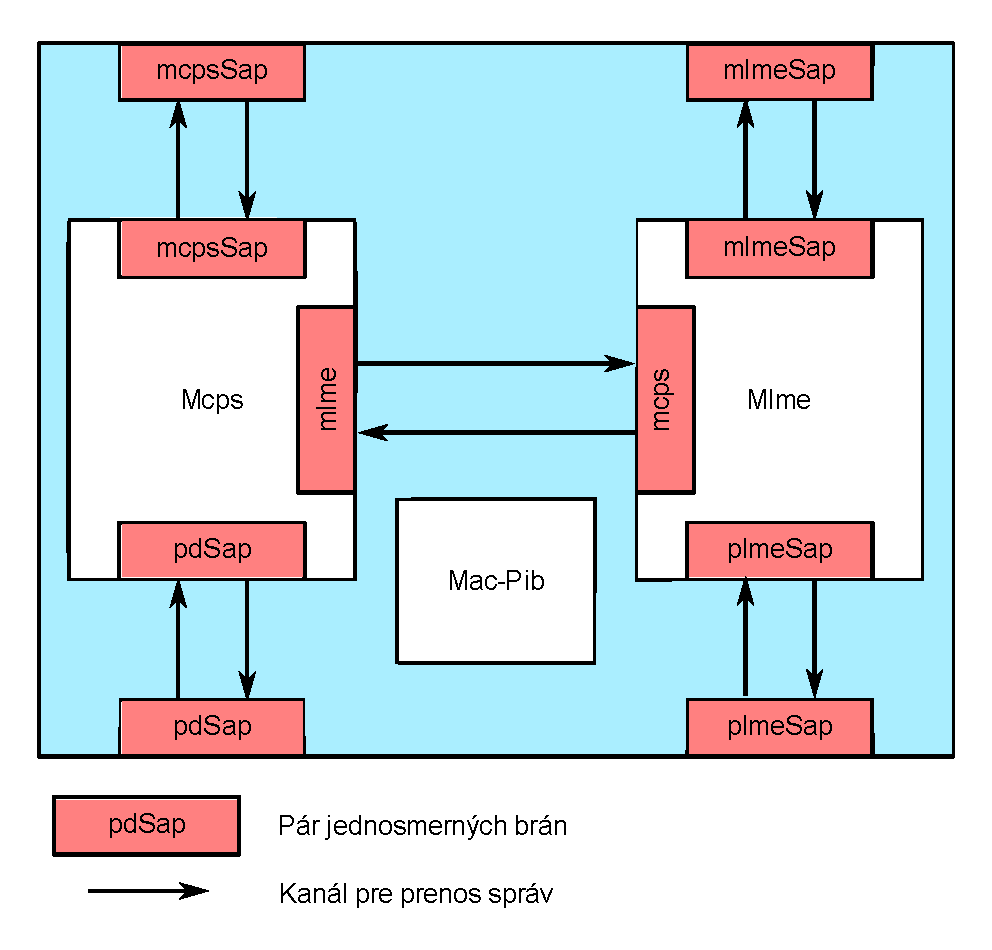
\includegraphics[width=120mm]{figures/architecture_mac}
\caption{Podoba implementovaného modelu linkovej vrstvy}
\label{fig:architecture_mac}
\end{center}
\end{figure}

\section{Fyzická vrstva - PHY}
\indent\indent Fyzická vrstva nášho modelu simuluje transformáciu bitov dodaných linkovou vrstvou na signál, ktorý je následne šírený médiom. Štandard pracuje so 7 komunikačnými módmi (obr. ~\ref{tab:frequencies}). Logika všetkých týchto módov je našim modelom podporovaná na strane komunikačných uzlov, ale pri začiatku simulácie sa musí nastaviť na jednu prenosovú frekvenciu \texttt{ChannelControl}. V tomto bude sa plánuje iný pohľad na správu spojení v simulátore MiXiM a tento nedostatok by sa mal odstrániť. Simulačný model by tam dovoľoval viacero aktívnych správcov spojení (moduly \texttt{ConnectionManager}). Úlohy fyzickej vrstvy sú alokované do 2 entít - analogicky ako aj v predošlých vrstvách: datovej (PD - PHY Data entity) a riadiacej (PLME - PHY Management Entity). Výs\-tupom smerom do éteru je bod služby RF-SAP a predstavuje rozhranie k rádiovému vysielaču/prijímaču.\\
\begin{figure}[htbp]
\begin{center}
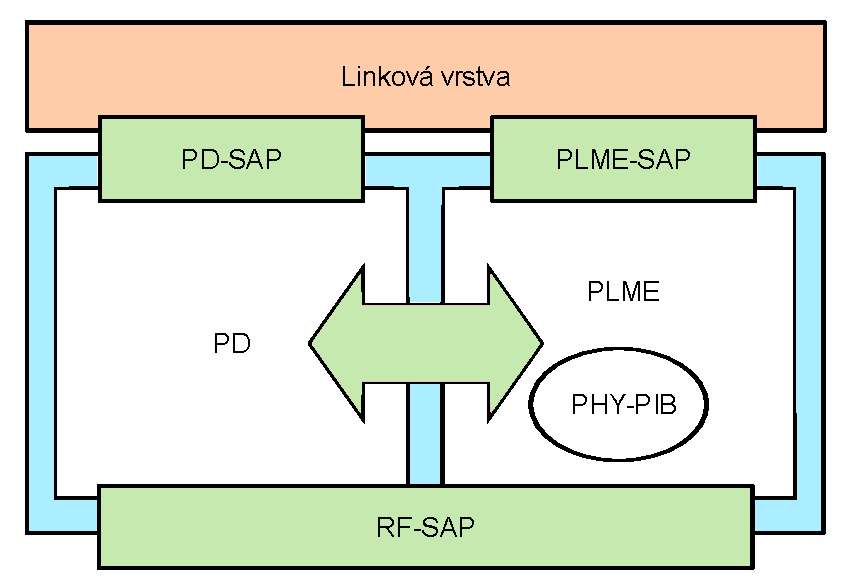
\includegraphics[width=120mm]{figures/topology_phy}
\caption{Referenčný model fyzickej vrstvy}
\label{fig:topology_phy}
\end{center}
\end{figure}
\subsection{Datová entita - PD}
\indent\indent Modul PD preposiela rámce medzi modulom \texttt{ChannelControl} a linkovou vrstvou cez bod prístupu PD-SAP. K rámcom pridáva dodatočné bity označované ako preamble a SFD bity (Starting Frame Delimiter). Tieto slúžia podľa špecifikácie k tomu, aby sa prijímací čip zosynchronizoval na týchto prijatých postupnostiach bitov. Vrstva PD nastavuje aj premennú \textit{lastMsgTimestamp}, ktorá je štruktúrou typu \textit{SimTime} a predstavuje časovú značku prijatých rámcov. Táto značka je nastavená až po prijatí bitov patriacich do preamble časti a SFD sekvencie. Názornejšie to vysvetľuje obr.~\ref{fig:frame_phy}.
\begin{figure}[htbp]
\begin{center}
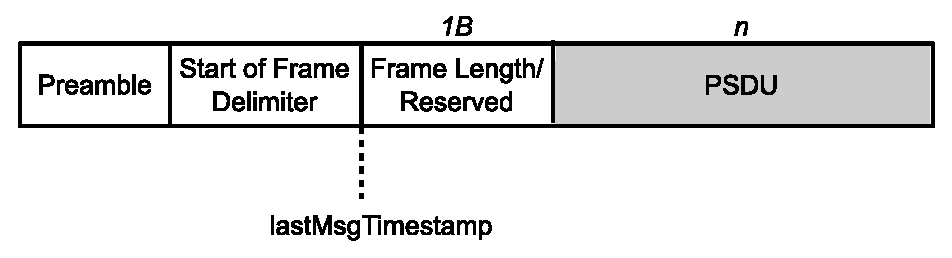
\includegraphics[width=140mm]{figures/frame_phy}
\caption{Spôsob enkapsulácie PSDU na fyzickej vrstve}
\label{fig:frame_phy}
\end{center}
\end{figure}
\paragraph{Implementácia}
Dĺžky polí preamble a SFD sa menia v závislosti od aktuálnej hodnoty \textit{phyCurrentChannel} a \textit{phyCurrentPage}. Sú zisťované priamo z modulu PHY-PIB (PHY layer Protocol Information Base). V tejto vrstve je to zatiaľ jediné miesto, kde je aktívne používaná utilita \texttt{Blackboard}. Pomocou nej sa vrstva PD dozvedá o tom, v akom stave je rádio a~aký je zámer MAC vrstvy (\textit{RX}/\textit{TX}). Podľa tejto informácie odosiela do bodu služby RF-SAP rámce.\\
\subsection{Riadiaca entita - PLME}
\indent\indent Riadiaca časť fyzickej vrstvy PLME má hlavne za úlohu spracovávať stavy rádia, prepínať ho na správnu frekvenciu a správny kanál. Úzko spolupracuje so sadou premenných a konštánt PHY-PIB. Vrstva ďalej informuje linkovú vrstvu o nameraných hodnotách pri ED (Energy Detection) snímaní okolia.\\
\paragraph{Implementácia}
Modul PLME je naprogramovaný tak, aby nedalo prípadnému záujemcovi veľa práce ho adaptovať na simulačný framework MiXiM. Tu sa nachádzajú úseky kódu, ktoré si budú vyžadovať úpravy k naplneniu cieľa. Jedná sa hlavne o zistenie spôsobu stavu energetickej hladiny kanálu. Tento údaj sa vysiela v primitíve PLME-ED-SCAN.confirm linkovej vrstve a v trochu inej podobe v primitíve PLME-CCA.confirm. V súvislosti s~ED skenovaním by bolo zaujímavé vedieť, aký je časový interval medzi prijatím správy PLME-ED-SCAN.request a odoslaním odpovede na ňu PLME-ED-SCAN.confirm. Pretože samotný údaj o dĺžke vykonávaného skenu je spracovaný linkovou vrstvou, ktorá o~tejto dĺžke neinformuje PLME modul, ale dovtedy opakuje vysielanie požiadavku na ED sken, dokedy jej nevyprší timer \textit{TIMER\_ED\_SCAN}. Následne modul MLME pracuje s~najvyššie zaznamenanou hodnotou vrátenou v správe PLME-ED-SCAN.confirm. Mimo to, modul PLME má za úlohu pristupovať do sady premenných a konštánt PHY-PIB za účelom predania ich hodnôt vyšším vrstvám cez primitívu PLME-GET.confirm, alebo ich nastavenia primitívou PLME-GET.request.\\
\indent Tento modul aj spracováva požiadavku pre vykonanie Clear Channel Assessment procedúry PLME-CCA.request. Za týmto účelom kontaktuje modul \texttt{SnrEval} a z neho vie zistiť, či je kanál v daný moment v stave \textit{IDLE}, alebo nie.\\
\begin{figure}[htbp]
\begin{center}
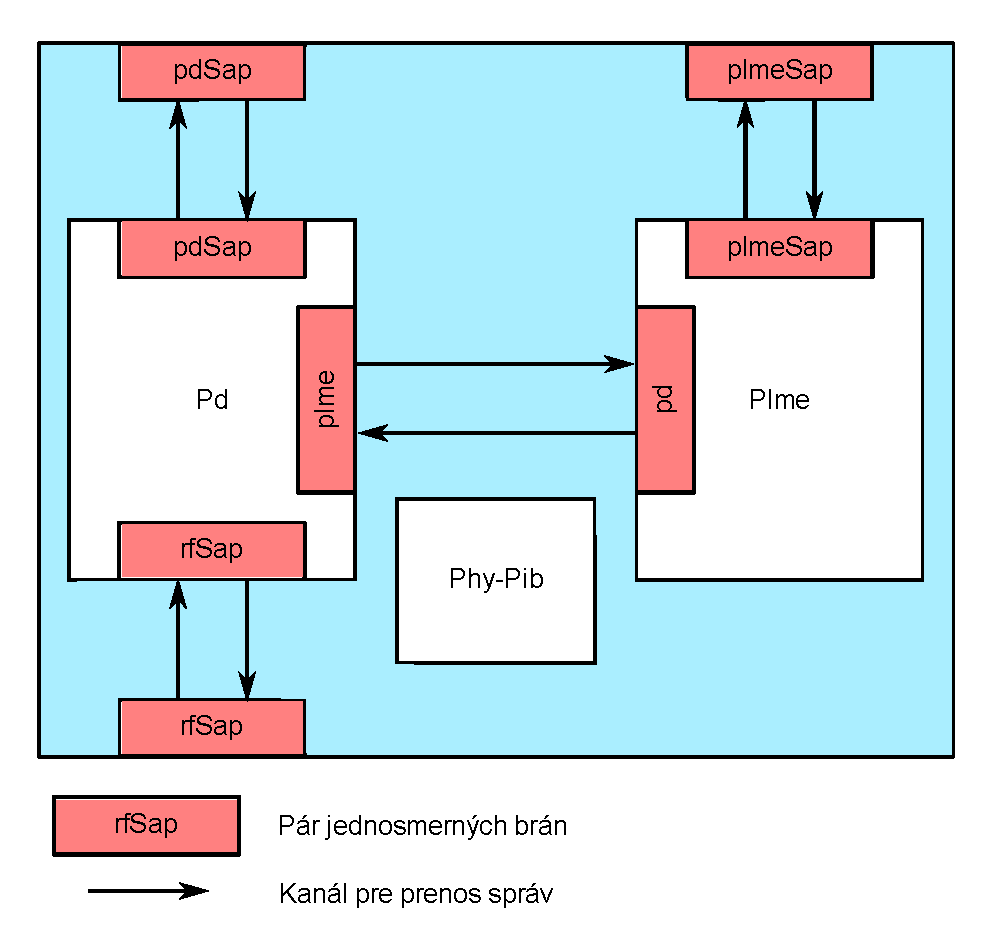
\includegraphics[width=120mm]{figures/architecture_phy}
\caption{Podoba implementovaného modelu fyzickej vrstvy}
\label{fig:architecture_phy}
\end{center}
\end{figure}
\subsection{Väzba na Mobility Framework}
\indent\indent Súčasťou fyzickej vrstvy v našom modeli sú už okrem spomenutých modulov aj moduly \texttt{SnrEval} a \texttt{SnrDecider}. Spôsob, akým zapadajú do architektúry modelu PHY je uvedený na obr.~\ref{fig:architecture_nic}. Tieto moduly sú súčasťou každej simulácie pod rozšírením Mobility Framework a v skutočnosti sú to upravené moduly z knižníc MF pre potreby nášho simulátora. Modul \texttt{SnrEval802154} vysiela rámce priamo modulu \texttt{ChannelControl}. V~opačnom smere, smere prijímania rámcov rozhoduje, či rámec sa príjme ako rámec, alebo je uvažovaný len ako príspevok k šumu. To závisí od toho, či je vypočítaná sila zaznamenaného signálu vyššia ako nastavená citlivosť prijímača. Energetická úroveň prijatého signálu sa počíta podľa vzorca$$P_{recv}=\frac{P_{send}\lambda^{2}}{16\pi^{2}l^{\alpha}}$$ kde $P_{send}$ znamená vyžarovací výkon, $\lambda$ vlnovú dĺžku nosnej, $\alpha$ predstavuje koeficient útlmu a $l$ vzdialenosť medzi zariadeniami. Modul \texttt{SnrEval802154} ďalej pracuje so stavom rádia a uverejňuje ho na \texttt{Blackboard}. V prípade spracovania správy ju pošle k modulu \texttt{SnrDecider802154}. Jeho úlohou je potom podľa úrovne SNR (Signal to Noise Ratio) a podľa prednastavenej hodnoty \textit{snrThreshold} prečítanej z modulu \texttt{ChannelControl} zistiť pravdepodobnosti chyby v prijatých rámcoch.\\
\indent Keď sa uvažuje vzduch ako spoločné prenosové médium, je potrebné si uvedomiť, že všetky zariadenia vzájomne sa ovplyvňujú. To znamená, že musia medzi nimi existovať spojenia. V prípade simulácie $n$ zariadení, počet spojení bude $n!$. Takýto prístup je pri svojom behu značne náročný na systémové prostriedky. V MF bola heuristickými metódami znížená táto náročnosť. Zadefinujme pojem interferenčná vzdialenosť. Jej hodnota bude predstavovať maximálnu prípustnú vzdialenosť medzi uzlami, pri ktorej ešte budeme uvažovať o ich vzájomnom rušení. Označme ju $r$. Vzdialenosť medzi uzlami označme $l$. Ak rozdelíme simulačnú plochu na štvorcové zóny s dĺžkou hrany $r$, môžme potom tvrdiť, že ovplyvňovať sa budú len uzly vrámci zóny a v vzájomne susediacich zónach. Uzly siete, ktoré sa nachádzajú vo vzdialenosti menšej, ako je interferenčná vzdialenosť ($l\in\langle0,r\rangle$), majú vytvorené medzi sebou spojenie. Uzly, ktoré sa nachádzajú vo vzdialenosti väčšej, ako je $2\sqrt{2}r$, spojenie určite vytvorené nemajú a~uzly, ktorých vzájomná vzdialenosť bude patriť do intervalu $l\in(r, 2\sqrt{2}r)$ budú mať spojenia vytvorené len v závislosti od ich polohy (viď obr.~\ref{fig:channelcontrol_areas}).\\
\indent Interferenčná vzdialenosť sa počíta podľa vzorca $$r=\left(\frac{\lambda^{2}P_{max}10^{3}}{16\pi^{2}10^{\frac{sat}{10}}}\right)^{\frac{1}{\alpha}}$$ kde $\lambda$ predstavuje vlnovú dĺžku nosnej frekvencie, $P_{max}$ najvyššiu hodnotu vyžarovacieho výkonu uzlu použitú v simulácii, premenná $sat$ hraničnú hodnotu útlmu (Signal Attenuation Threshold) a $\alpha$ koeficient útlmu. Pre nami použité hodnoty $\lambda=0,125$ ($f=2,4.10^{9}[Hz]$), $P_{max}=10\cdotp10^{-3}[mW]$, $sat=-112[dBm]$ a $\alpha=3,5$ vychádza hodnota interferenčnej vzdialenosti $r=219.555[m]$.\\
\indent V grafickom okne bežiacej simulácie (obr.~\ref{fig:screen_init} a obr.~\ref{fig:screen_beacons}) je dobre vidieť, aký výsledok sa dostaví s použitím uvedenej heuristiky pri pri nastavení prostredia podľa vyššie uvedených hodnôt parametrov. Spojenia sú vytvorené len medzi určitými uzlami a dynamicky vznikajú a zanikajú počas behu simulácie v závislosti na pohybe sieťových prvkov po ploche. V danom prípade bola nastavená dĺžka strany simulačného poľa o veľkosti $500m$.\\
\begin{figure}[htbp]
\begin{center}
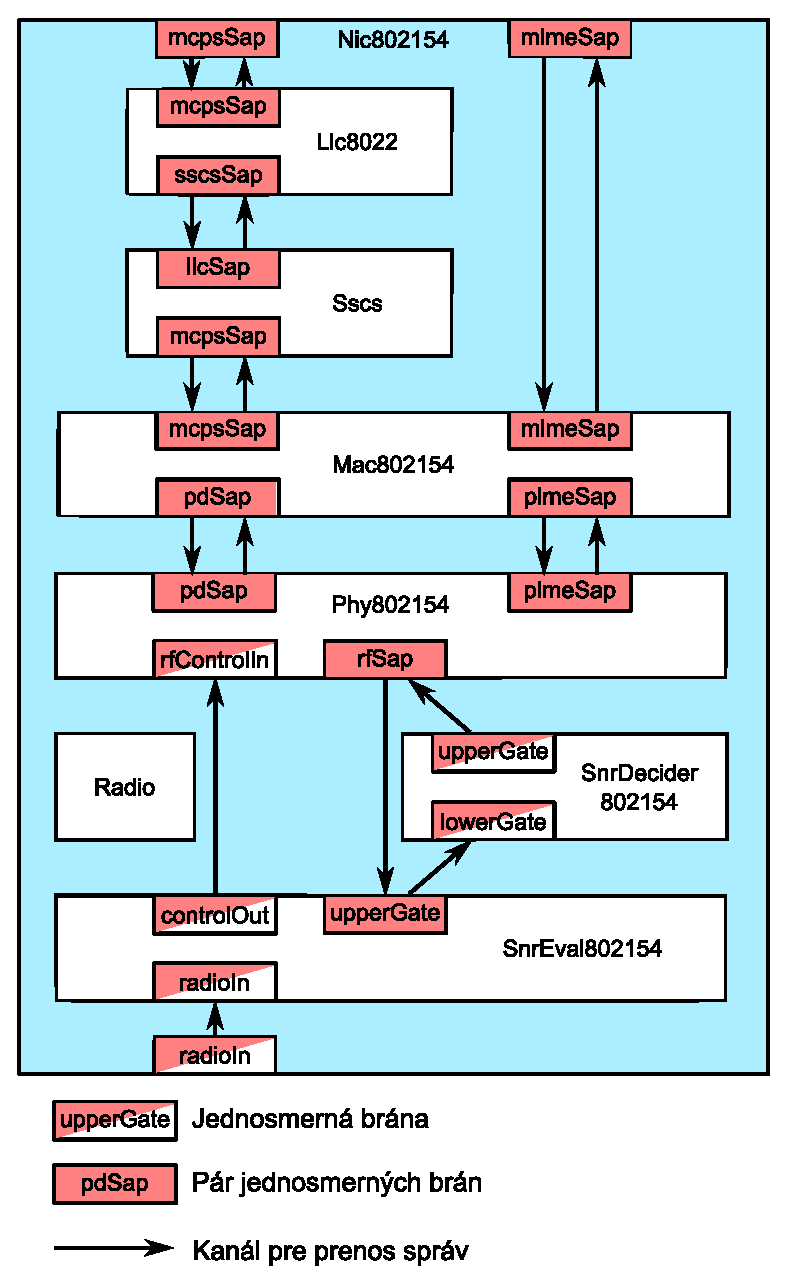
\includegraphics[width=120mm]{figures/architecture_nic}
\caption{Modul rozhrania 802.15.4 a jeho štruktúra v kontexte s rozšírením Mobility Framework}
\label{fig:architecture_nic}
\end{center}
\end{figure}

\section{Mobilita}
\indent\indent Mobility Framework poskytuje, ako už z jeho názvu vyplýva, silnú podporu mobilite modelov. V MF je mobilita rozdistribuovaná medzi všetky moduly FFD a RFD. Keďže nie je dôvod, aby jeden prvok ovplyvňoval druhý v pohybe, mobilita je počítaná na lokálnej úrovni jednotlivých prvkov. Informácia o vzájomných polohách zariadení je potom spracovávaná v module \texttt{SnrDecider} z informácii, ktoré poskytne \texttt{ChannelControl}. Mobility Framework 2.0 preview 3 má obsiahnutých niekoľko základných modelov pohybu po simulačnom poli. K základným patria:\\
\paragraph{CircleMobility} kde prvok opisuje trajektóriu v tvare kružnice s definovaným stredom, polomerom, rýchlosťou, počiatočným uhlom zvierajúcim sprievodiča s osou X (\textit{startAngle}) a periodicitou updatovania danej polohy. Obdobne pracuje aj model \textbf{RectangleMobility}, ktorý definuje pohyb po obdĺžniku.
\paragraph{ConstSpeedMobility} je mobilita, ktorá simuluje pohyb zariadenia smerom k náhodne definovaným cieľom s konštantnou rýchlosťou. Po dosiahnutí tohoto konkrétneho cieľa je ďalej zvolený iný, tiež náhodný.
\paragraph{LinearMobility} modeluje pohyb po poli s definovaným počiatočným stavom (súradnice, uhol pohybu voči osi X, rýchlosť a zrýchlenie). Smer pohybu prvku sa potom zmení len pri dosiahnutí okraja poľa, na ktorom prebieha simulácia, a to podľa pravidla uhol dopadu $=$ uhol odrazu.
\paragraph{MassMobility}~\cite{massmobility99} opisuje nasledovný spôsob pohybu po poli: prvok sa pohybuje priamo po priamke po dobu náhodne dlhého intervalu. Dĺžka toho intervalu je daná normálnym rozložením. Po uplynutí tohoto intervalu zmení smer pohybu o uhol, ktorého veľkosť je tiež náhodné číslo z normálneho rozloženia. Zároveň zmení v tomto bode aj rýchlosť na nejakú náhodnú veľkosť. Po náraze na hranicu simulačnej zóny sa odrazí pod rovnakým uhlom. Tento model hovorí o tom, že prvky majú moment zotrvačnosti a nemenia smer pohybu nárazovo. Východzie hodnoty sú $changeInterval = normal(5, 0.1) [s]$, $changeAngleBy = normal(0, 30) [deg]$ a $speed = normal(avgSpeed, 0.01) [m/s]$.
\paragraph{TurtleMobility} modul spracováva pohyb opísaný externýmn súborom vo formáte *.xml. Pohyb je nadefinovaný určitými blokmi úsekov, ktoré majú zadanú počiatočnú zmenu smeru, rýchlosť a číslo, koľko krát sa danú blok opakuje.\\ \\
\indent Mobility modely v MF sú aj schopné pracovať s externe definovanými modelmi mobility simulátora \textbf{ANSim}~\cite{ansim_report} a s modelmi mobility formátu \textbf{BonnMotion}~\cite{bonnmotion_report}. Všetko závisí na tom, aký spôsob mobility architektúry je definovaný v súboroch \texttt{FFD.ned} a~\texttt{RFD.ned}.\\
\indent V simulátore MiXiM bude obsiahnutý podobný prístup k riešeniu mobility prvkov. Tam bude existovať aj centrálny prvok riadiaci mobilitu a eventuelné kolízie prvkov \texttt{ObjectManager}. Predpokladá sa, že množstvo mobility modelov z MF bude implementované aj do MiXiM frameworku.\\

\section{IP over IEEE 802.15.4}
\indent\indent Až donedávna bola predstava, že IP prístup bude obchádzať LR-WPAN siete, pretože IP protokoly nebude možné preškálovať na linky s nízkymi prenosovými rýchlosťami, z~ktorých množstvo funguje v energeticky úsporných režimoch. IEEE 802.15.4 rámce sú relatívne malé a celý stack protokolov sa musí zmestiť do obmedzeného pamäťového priestoru. Návrh štandardu IETF 6LoWPAN pre IPv6 komunikáciu~\cite{rfc_4919} a~\cite{rfc_4944} cez IEEE 802.15.4 zmenil pohľad na danú problematiku. S podporou šifrovania AES-128 zahrnul základné bezpečnostné a autentizačné mechanizmy. Uvedený štandard definuje spôsob prenosu IP paketov cez siete štandardu IEEE 802.15.4 vďaka čomu umožňuje interoperabilitu medzi zariadeniami na rôznych linkách v hierarchii siete a zároveň dovoľuje paralelné fungovanie zariadení v týchto sieťach, ktoré nepoužívajú IP pakety k prenosu dát.\\
\indent Nasadenie IP technológie nad IEEE 802.15.4 má mnohé výhody. Menovite odpadá veľké množstvo potrebných smerovačov rôznych IEEE 802.15.4 protokolov, riadiacich a~bezpečnostných procedúr, pretože v týchto veciach sa môžme spoľahnúť na protokoly z rodiny TCP/IP. Nevýhodou nasadenia IPv6 sú veľké polia v hlavičke paketu a~spolu s~užitočným obsahom paketu presahujú prípustné veľkosti rámcov IEEE 802.15.4 (IPv6: 1280 B, 802.15.4: max 127B). 6LoWPAN formát v základnom režime pracuje s extrémne kompaktným záhlavím IP, ktoré rozširuje v prípade, že viaceré vlastnosti a schopnosti IPv6 protokolu sú využívané. Napríklad pri komunikácii susediacich 802.15.4 zariadení, polia obsahujúce IP adresy môžu byť skrátené takmer na nulu. V plnej forme sú použité v prípade, že jeden koniec komunikačného toku sa nachádza mimo 802.15.4 siete. Pri prekročení veľkosti MPDU, ktorú sú schopné zariadenia preniesť, sa pristupuje k~fragmentácii. Tiež návrh 6LoWPAN dovoľuje smerovať rámce pomocou IP v sietiach LR-WPAN. Senzorové siete budú obsahovať brány (gateways), ktorých funkcionalita bude zredukovaná na úlohu jednoduchého smerovača medzi senzorovou a konvenčnou sieťou. Je nutné poznamenať, že IEEE 802.15.4 neposkytuje podporau pre broadcast smerovanie, čo sa samozrejme negatívne prejaví prina fungovaní protokolu IPv6, ktorý práve poskytuje silné mechanizmy na prácu s broadcast a multicast adresami. Z absencie broadcast smerovania sa nedá počítať s fungovaním služieb vyžadujúcich broadcast komunikáciu ako napr. DHCP (Dynamic Host Configuration Protocol).\\
\begin{figure}[htbp]
\begin{center}
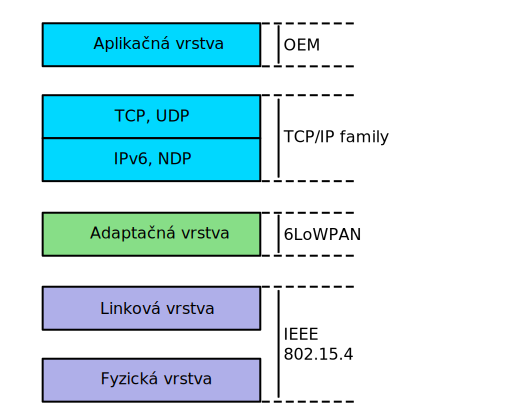
\includegraphics[width=120mm]{figures/ip_ieee}
\caption{Architektúra modulu komunikujúceho IP protokolmi na LR-WPAN sieti}
\label{fig:ip_ieee}
\end{center}
\end{figure}
\indent Pre nasadenie IP komunikácie je pripravené rozhranie na linkovej vrstve, ktoré poskytuje adaptačnej vrstve vstupné brány \texttt{input mlmeSapIn}, \texttt{input mcpsSapIn} a výstupné \texttt{output mlmeSapOut}, \texttt{output mcpsSapOut}. Modul linkovej vrstvy je implementovaný tak, aby korektne spracoval sekvencie správ pre inicializáciu siete (správy typu MLME-BEACON-NOTIFY.indication, MLME-SCAN.request, MLME-START.request, MLME-ASSOCIATE.request, MLME-SET.request). Tieto správy sú postačujúce na to, aby sa adaptačný modul nakonfiguroval pre správne prenášanie paketov IP, zviazal IPv6 s 64-bit IEEE adresami a bol schopný enkapsulovať IP pakety do IEEE 802.15.4 rámcov. Presné definície a formáty správ, cez ktoré je možné naviazať adaptačnú vrstvu k~linkovej vrstve sú uvedené v súbore \texttt{Messages.msg} a~majú prefix \texttt{Mlme}.
